\documentclass[14pt]{extarticle}

\let\Overrightarrow\overrightarrow
\let\vecarrow\overrightarrow

%other%
\usepackage{graphicx}
\usepackage{float}
\usepackage[margin=0.7in]{geometry}
\usepackage{caption}
\usepackage{csquotes}
\usepackage[export]{adjustbox}
\usepackage{wrapfig}
\usepackage{setspace}
\usepackage{anyfontsize}
\usepackage{titlesec}
\titleformat{\section}{\normalfont\fontsize{20}{20}\bfseries}{\thesection}{1em}{}
\titleformat{\subsection}{\normalfont\fontsize{17}{20}\bfseries}{\thesubsection}{0.1em}{}
\usepackage{relsize}
\usepackage{indentfirst}
\usepackage{lipsum}
\usepackage{fancybox,framed}
\usepackage{comment}
\usepackage{enumitem}
\usepackage{biolinum}
%other%


%math%
\usepackage[fleqn]{amsmath}
\usepackage{amsthm}
\usepackage{nccmath}
\usepackage{amsmath}
\usepackage{amssymb}
\usepackage{mathtools}
\usepackage{yfonts}
%\usepackage{BOONDOX}

\usepackage{unicode-math}
\setmathfont{Latin Modern Math}

%\usepackage{unicode-math}
%\newtheorem*{}{\textup{Лемма}}
\newtheoremstyle{definition}
{3pt}
{3pt}
{\upshape}
{}
{\itshape\bfseries\fontsize{15}{15}}
{.}
{.5em}
{}
\theoremstyle{definition}
\newtheorem*{definition}{Определение}


%\newtheorem*{theorem}{\normalfont\fontsize{15}{15}\textup{Теорема}}
\newtheoremstyle{theorem}
{3pt}
{3pt}
{\itshape}
{}
{\bfseries\upshape\fontsize{15}{15}}
{.}
{.5em}
{}
%{\thmname{#1}\thmnumber{ #2}\thmnote{ (#3)}}

\theoremstyle{theorem}
\newtheorem*{theorem}{Теорема}

%\newcommand

%\newtheorem*{named}{\innerheader}

\newenvironment{namedtheorem}[2]
{
\newcommand{\foo}{#1}
\newtheorem*{\foo{}}{\normalfont\fontsize{15}{15}{Теорема #2}}
\begin{\foo{}}
}
{\end{\foo{}}}

%\newtheoremstyle{named}{}{}{\itshape}{}{\bfseries}{.}{.5em}{\thmnote{#3's}#1}
%\theoremstyle{named}
%\newtheorem*{namedtheorem}{theorem}
\newtheorem*{remark}{\textup{Комментарий}}
%\renewcommand\qedsymbol{$\blacksquare$}
%\usepackage{parski}
\renewenvironment{proof}
    {\noindent \textit{Доказательство.}\\
	\indent $\square$}
	{ $\blacksquare$\\ }

\newenvironment{solution}
	{\noindent\textbf{Решение.}}


\renewenvironment{remark}
    {\noindent\textbf{Комментарий.}}

\newenvironment{note}
    {\noindent {\normalfont\fontsize{14}{14}\textbf{\textit{Примечание.}}}}


\usepackage{tikz}
   \usetikzlibrary{calc}

\newcommand{\arc}[0]{
   \tikz [baseline = (N.base), every node/.style={}] {
	  \node [inner sep = 0pt] (N){}; %{$#0$};
      \draw [line width = 0.8pt] plot [smooth, tension=1.3] coordinates {
         ($(N.north west) + (-1.5ex,0.6ex+0.4ex)$)
         ($(N.north)      + (-0.75ex,0+0.4ex)$)
         ($(N.north east) + (0ex,0.6ex+0.4ex)$)
      };
   }
}

\renewenvironment{rcases}
  {\left.\begin{aligned}}
  {\end{aligned}\right\rbrace}

\DeclarePairedDelimiter\abs{\lvert}{\rvert}
\DeclarePairedDelimiter\norm{\lVert}{\rVert}


%\newcounter{example}[section]
\newenvironment{example}[1]{\noindent \textbf{Пример #1.}}
%\newcommand{\mathleft}{\mathindent0pt}
%{\@fleqntrue}
%\@mathmargin0pt}
%math%

%fonts%
\usepackage[russian]{babel}
\usepackage{polyglossia}
\setdefaultlanguage[spelling=modern]{russian}
%\setotherlanguage{english}
\setmainfont{CMU Serif}
\setsansfont{CMU Sans Serif}
\setmonofont{CMU Typewriter Text}  
%\setmathfont{Latin Modern Math}



\begin{document}

\noindent \textbf{Задача 1.} \quad
Пусть \(\Gamma\) --- окружность, описанная около остроугольного 
треугольника \(ABC\). Точки \(D\) и \(E\) лежат на отрезках \(AB\) 
и \(AC\) соответственно, причем \(AD = AE\). Серединные перпендикуляры 
к отрезкам \(BD\) и \(CE\) пересекают меньшие дуги \(AB\) и \(AC\) 
окружности \(\Gamma\) в точках \(F\) и \(G\) соответственно. Докажите, 
что прямые \(DE\) и \(FG\) параллельны или совпадают. \\

\begin{solution}
Пусть \(FG\) пересекает \(AC\) и \(AB\) в точках \(P\) и \(Q\) 
соответственно. \\Тогда для того, чтобы прямые \(DE\) и \(FG\)
были параллельны достаточно показать, что треугольник \(APQ\) является 
равнобедренным, то есть \(\angle APQ = \angle AQP\).
Положим \(\angle DAF = \varphi\), \(\angle EAG = \gamma\), 
\(\angle FDB = \angle FBD = \alpha\), \(\angle GEC = \angle GCE = \beta\).
Тогда \(\angle AQP = \dfrac{1}{2} ( \arc FB + \arc AG ) 
= \varphi + \beta\) и \(\angle APQ = \dfrac{1}{2} 
( \arc GC + \\ + \arc AF ) =  \alpha + \gamma\). То есть надо 
доказать, что \( \gamma + \alpha = \beta + \varphi \). Заметим, что 
\(\alpha = \varphi + \angle DFA\) (как внешний к \(\triangle ADF\)) 
и \(\beta = \gamma + \angle EGA\) (как внешний к \(\triangle AGE\)). 
Таким образом, задача свелась к равенству углов \(\angle DFA\) и 
\(\angle EGA\).

\begin{figure}[H]
	\centering
    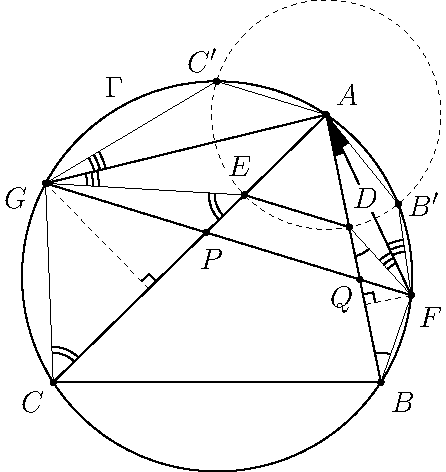
\includegraphics[height=10cm]{./img/problem_1.pdf}
\end{figure}

Пусть \(B' \in \Gamma\) и \(C' \in \Gamma\) так, что 
\(G\) и \(F\) середины дуг 
\(\arc CC'\) и \(\arc BB'\) соответственно. Покажем, что \(AD = AB'\).
Для начала заметим, что \(AF\) --- биссектриса угла \(\angle BAB'\).
Значит, симметрично 
отразив прямую \(AB\) относительно \(AF\), мы 
получим прямую \(AB'\). Пусть тогда \(D\) перейдет в \(D'\), тогда 
\(FD = FD'\). Заметим, что \(\angle ADF = 180^{\circ} - \angle FDB = 
180^{\circ} - \angle FBD = 180^{\circ} - \angle AGF = \angle AB'F\). 
Следовательно, \(D' = B'\), а значит \(AD = AD' = AB'\). 
Аналогично доказывается, что \(AE = AC'\). Тогда \(AB' = AD = AE = AC'\).
Отсюда мгновенно cледует, что \(\angle DFA = \angle D'FA = \angle B'GA 
= \angle EGA\). Это нам и требовалось.
%Тогда точка \(D'\) --- одна из точек пересечения прямой \(AB'\) и 
%окружности с центром \(F\) и радиусом \(FD\). Очевидно, что угол 
%\(\angle ADF\) -- тупой, так как смежный с ним угол 
%\(\angle FDB = FBD = \dfrac{1}{2} \arc AF < \dfrac{1}{2} \arc AB = 
%\angle C < 90^{\circ}\). Остается заметить, что угол \(\angle AB'F = 
%180^{\circ} - \angle AGF\) --- также тупой, так как \(\angle AGF \)
\end{solution}

\end{document}
